% Chapter 1

\chapter{Introduction} % Main chapter title

\label{Chapter1} % For referencing the chapter elsewhere, use \ref{Chapter1} 
%----------------------------------------------------------------------------------------

% Define some commands to keep the formatting separated from the content 
\newcommand{\keyword}[1]{\textbf{#1}}
\newcommand{\tabhead}[1]{\textbf{#1}}
\newcommand{\code}[1]{\texttt{#1}}
\newcommand{\file}[1]{\texttt{\bfseries#1}}
\newcommand{\option}[1]{\texttt{\itshape#1}}


%----------------------------------------------------------------------------------------
% Motivation and Background
\section{Motivation}
% - motivate topic models
% data is big
Researchers today are faced with a deluge of data. As we continue to digitize and aggregate our collective knowledge we produce ever increasing archives of information. The sheer volume and variety of forms this information may take - text, images, audio, video, social connections etc. - makes it difficult and in most cases impossible to parse manually. 

% need better tool
This driving factor of data growth has given rise to internet giants such as Google, Yahoo, and Baidu that help us access and browse pre-indexed swathes of information. However in order to go beyond mere keyword searches, or link analysis, and break into the realm of understanding each document, requires a new approach to data exploration.

% Topic modeling is that tool
A powerful set of computational tools referred to as probabilistic topic models have emerged to meet this challenge. Aimed to discover and annotate large archives of documents with thematic information, topic models identify patterns that reflect the underlying topics which combined to form those documents.

% it can do things unsupervised (so it can automate)
Naturally, it is rare that we would know beforehand exactly what topics a given document contains, and thus topic modeling constitutes an unsupervised task. As a result, topic modeling algorithms are designed to work without prior knowledge of the topic distribution of a given document — that is, the topics are derived from the texts themselves. This makes the organization, summarization and annotation of text corpora possible at an inhuman scale. Consequently, topic models are useful in a variety of settings and have successfully been applied to web archives, news articles \parencite{Newman:2006:AET:2106961.2106971}, and academic literature \parencite{Steyvers:2004:PAM:1014052.1014087} to elicit insight. In this paper, we focus our experiments on extracting topics from patent data with the hopes identifying meaningful trends in renewable energy technologies. 

% we use patent data because they offer a rich corpus of science and engineering, ebcause patents show how innovation has progressed. Extracting topics will be meaningful.

%hidden/latent thematic structure in large archives of documents.
%vast quantities of unstructured data
%large databases of text
%electronic document archives
%collections of text


%----------------------------------------------------------------------------------------
\section{Primer on Latent Dirichilet allocation} \label{ldaprimer}
% - Intuitive explanation (distribution over topics)
Fortunately, the intuition behind LDA topic models is relatively straight forward. To understand how the algorithm infers the topics in relation to documents we first define what constitutes a topic. A topic is a distribution over a fixed vocabulary, where each word has an assigned probability of occurrence. Subsequently, we can take the view that each document is likely a product of one or more topics, a cocktail of themes as it were with different proportions of each ingredient.

% EPO Worldwide Patent Statistical Database
% example with topic words highlighted
Take for example the following document sampled from the August 2014 EPO Worldwide Patent Statistical Database (\keyword{PATSTAT}). The patent abstract contained in Figure \ref{fig:Patent_114} relates to a mechanism for stopping a water wheel. We have taken the liberty of highlighting a selection of words from a few of this document's prominent topics. Words like 
"pressure", "liquid", and "flow" belong to the \keyword{fluids/water} topic and are colored blue. While words relating to the \keyword{mechanisms} by which this fluid is directed such as "chamber", "valve", and "guide" are colored red. Finally, words such as "transmission", "speed", and "operated" belong to the topic associated with \keyword{signals} and are colored green.

\begin{figure}[h]
\centering
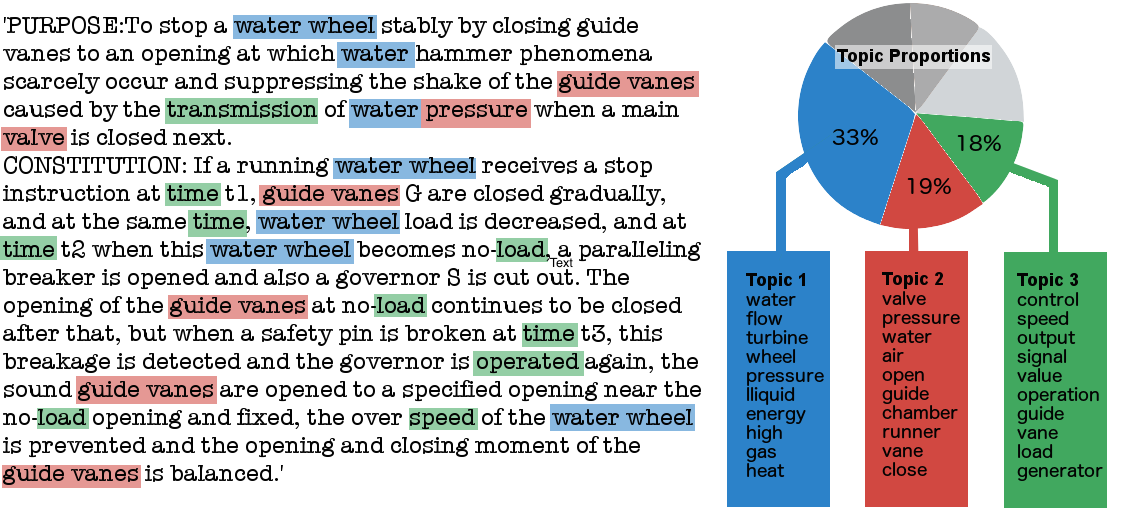
\includegraphics[width=130mm,scale=0.45]{Figures/Patent114}
\decoRule
\caption[Patent114]{Topic proportions in a sample patent abstract.}
\label{fig:Patent_114}
\end{figure}

The topics in the previous example were formed not over a single document but over a collection. The grey sections of the pie chart above represent the topics that this patent does not contain strong elements of. This is a key characteristic of LDA topic models, each document has a unique topic 'fingerprint' as a result of a generative process. That process for generating a document word by word is as follows. First we decide, sampling from the distribution of topics, which topic our first word will belong to. Then we sample from that chosen topic's distribution to decide what the word itself will be. This process is then simply repeated for each word, and while it works it has the following assumptions worth noting:

% assumptions
\begin{itemize}
\item Documents can manifest multiple topics (however typically not many)
\item Each document is assumed to be the product of a generative process.
\item Generative process starts with a topic, i.e. a distribution over a fixed vocabulary.
\item Assumes a fixed number of topics
\end{itemize}

% math framework.
Latent Dirichilet allocation falls into a family of machine learning algorithms called \keyword{hidden variable models}.  In this family of models, the user customarily "posits a hidden structure in the observed data, and then learns that structure using posterior probabilistic inference" \parencite{TopicModels2009}. For LDA specifically, the documents are the observed data, the topics and document topic proportions are hidden.

More formally, we may define this process mathematically as a joint distribution over our hidden variables and our observed variables. Specifically, we define the distribution over vocabulary as $\beta$, the topic proportions for document d $\theta_d$, the topic assignment for a word in a document $z_{d,n}$ and of course the observed words themselves $w_{d,n}$. 

\begin{align*}
  & P(\beta_{1:K},\theta_{1:D},z_{1:D},W_{1:D}) \nonumber \\
  & = \prod_{i=1}^K p(\beta_i) 
  \prod_{d=1}^D p(\theta_d)
  \{ \prod_{n=1}^N p(z_{d,n}|\theta_d)p(w_{d,n}|\beta_{1:k},z_{d,n}) \} \numberthis \label{eq:JointProb} 
\end{align*}

In Eq \ref{eq:JointProb} we see a few dependencies worth noting. Firstly that the topic we assign to a word $z_{d,n}$ depends on the distribution of topics of its document $\theta_d$. Additionally, that the identity of the word itself is dependent on not only the topic we assigned to generate it $z_{d,n}$, but also the vocabulary distributions of each topic $\beta_{1:K}$. Equivalently we can express the dependencies between these variables as a graphical model, illustrated in figure \ref{fig:Gmod1}.

\begin{figure}[ht]
\centering
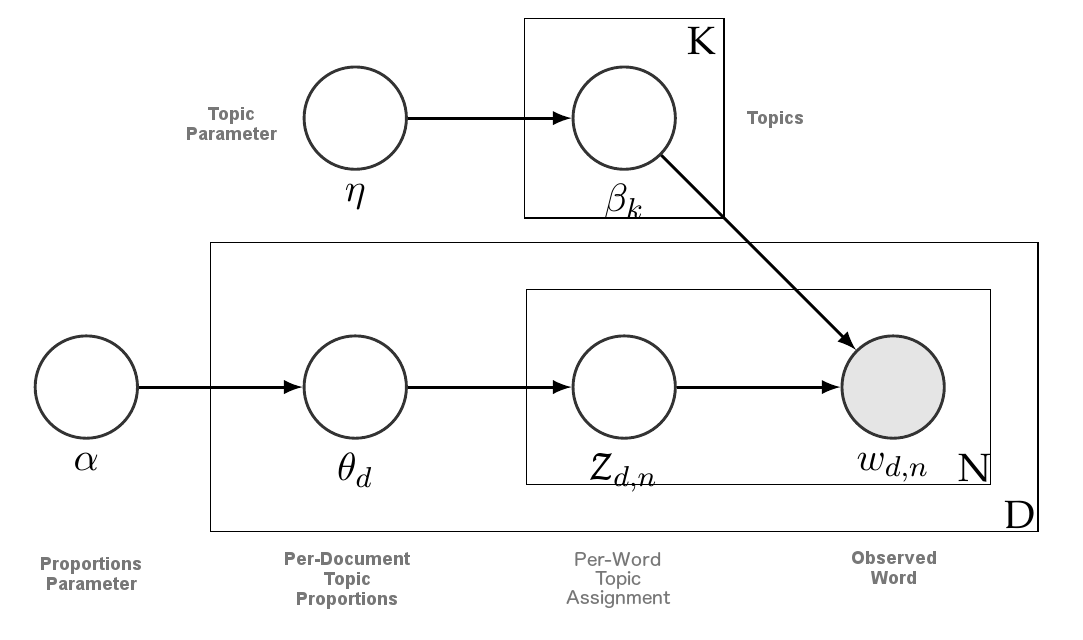
\includegraphics[width=130mm,scale=0.45]{Figures/gmod1}
%\begin{tikzpicture}
%\tikzstyle{main}=[circle, minimum size = 10mm, thick, draw =black!80, node distance = 16mm]
%\tikzstyle{connect}=[-latex, thick]
%\tikzstyle{box}=[rectangle, draw=black!100]
%  \node[main, fill = white!100] (alpha) [label=below:$\alpha$] { };
%  \node[main] (theta) [right=of alpha,label=below:$\theta_d$] { };
%  \node[main] (T) [right=of theta,label=below:$T_{d,n}$] {};
%  \node[main] (eta) [above=of theta,label=below:$\eta$] { };
%  \node[main, fill = black!10] (w) [right=of T,label=below:$w_{d,n}$] { };
%  \node[main] (beta) [above=of T,label=below:$\beta_k$] { }; 
%  \path (alpha) edge [connect] (theta)
 %       (theta) edge [connect] (T)
  %      (T) edge [connect] (w)
  %      (beta) edge [connect] (w)
  %      (eta) edge [connect] (beta);
%  \node[rectangle, inner sep=0mm, fit= (T) (w),label=below right:N, xshift=13mm] {};
%  \node[rectangle, inner sep=4.4mm,draw=black!100, fit= (T) (w)] {};
 
%  \node[rectangle, inner sep=4.6mm, fit= (theta) (T) (w),label=below right:D, xshift=26.0mm] {};
%  \node[rectangle, inner sep=9mm, draw=black!100, fit = (theta) (T) (w)] {};
  
%  \node[rectangle, inner sep=4.6mm, fit= (beta),label=above right:K, xshift=-5.0mm, yshift=-5.0mm] {};
%  \node[rectangle, inner sep=4.6mm, draw=black!100, fit = (beta)] {};
%\end{tikzpicture}
\caption{Graphical model for LDA}
\label{fig:Gmod1}
\end{figure}

So how do we actually obtain our estimates of the hidden parameters? We need to calculate the conditional distribution of our hidden parameters (the topic structure), and the observed words i.e. the posterior distribution described in Eq. \ref{eq:LDAPost}. However the denominator makes this calculation computationally infeasible due to the number of combinations our hidden parameters could take. 

\begin{align}
  p(\beta_{1:K},\theta_{1:D},Z_{1:D}|W_{1:D}) = \frac{p(\beta_{1:K},\theta_{1:D},Z_{1:D}|W_{1:D})}{p(W_{1:D})} \numberthis \label{eq:LDAPost}
\end{align}

To move past this, most solutions use either sampling or variational based methods to perform approximate inference and obtain estimates of the hidden parameters. Variational methods allow us to translate the original problem to one of optimization and take advantage of the many optimization techniques available. This in turn allows us to make extensions that are often faster, scale better or allow for different forms of input such as streaming documents. 


%----------------------------------------------------------------------------------------
\section{Adding a temporal component}
% how is the DTM different?
One such extension, and the extension we explore in this study, is to relax the implicit assumption of LDA that the order of the documents doesn't matter. 
By incorporating the order of the documents to the model, a topic is no longer simply a distribution over words but now becomes a \emph{sequence} of distributions over words. This is the jump that allows us not only to identify a theme, as with static LDA, but also track how it progresses in time, giving us the Dynamic Topic Model (\keyword{DTM}).

%this is friggin' cool and you should be interested because it allows us to do some awesome stuff.
% - describe how a dynamic model might improve on the "normal" LDA
% - describe the usefulness of having a temporal component in the model. (maybe give specific example documents)
The DTM offers several advantages over traditional LDA including improved predictive performance \parencite{Blei:2006:DTM:1143844.1143859}. Primarily though, it facilitates a greater understanding of how each topic developed, and how the ideas therein formed and matured. With it, we can inspect trends of word usage to uncover a richer and more detailed hidden structure. For instance figure \ref{fig:wwttTopic6} contains a sample theme from a sub-collection of hydroelectric patents and the progression of word prevalences within it over time.

% super quick example
\begin{figure}[ht]
\centering
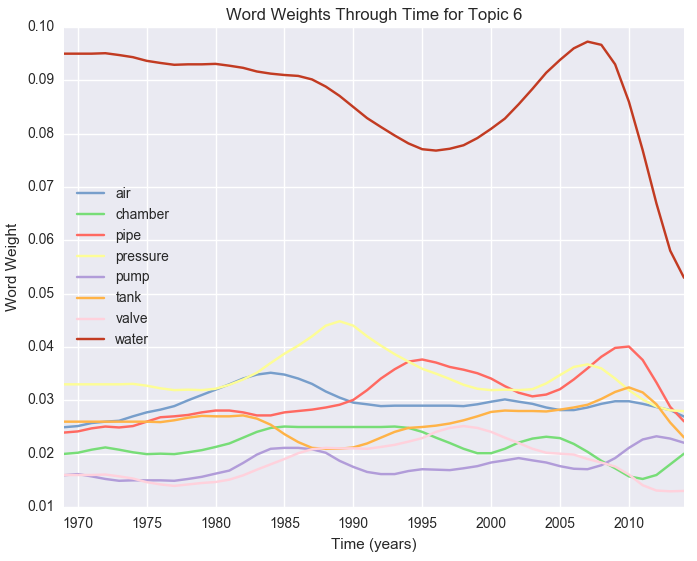
\includegraphics[width=130mm,scale=0.45]{Figures/wwttTopic6}
\decoRule
\caption[wwttTopic6]{Distribution over words in a sample hydroelectric topic over time}
\label{fig:wwttTopic6}
\end{figure}

%high level quick overview of the math? Or save it for the DTM section...
% DIDNT EVEN MENTION THE DIM!!!

%---modeling influence------
%\section{Modeling Influence}
% influence measurements of scientific journals and articles help determine decisions about funding and publishing. Traditionally this is done using citations (Garfield 2002) with the intuition that if more people cite a work, it is likely to be more influential.

% while scientific papers and in our case patents contain citations many texts don't such as news, blogs, legal documents.

% all citations are also counted equally as having contributed to a work which is rarely the case.

% new intuition that an influential paper will affect the language of subsequent related papers in a variable manner.

% DIM is the sibling of DTM



%----------------------------------------------------------------------------------------
\section{Why patents?}
% - reference why applying it to patents is not an accident. 
% i.e. why patents provide an interesting use case.
Patent data is specifically interesting in this context because of the role patents play in company formation, job growth, economic development, and novel invention. Their history tells a story of technological progression. In an attempt to maintain a competitive edge, many companies large and small spend a considerable amount of energy researching this history to identify technical trends relevant to their industry. 

% what's even more cool, is applying that DTM to patent data. we can effectively track the progression of innovation through language use in patent abstracts. 
Dynamic topic models have the potential to aid this research by enabling us to track the evolution of innovation through language use in patent abstracts. In this paper we look at a number of elements, including the evolution of technological themes and their proportions, the origination and development of language, as well as document influences. Furthermore, the patent corpus and associated International Patent Classification (\keyword{IPC}) labels provide a platform for the comparison of various topic modeling algorithms.

%research into new products or industries does not occur in a vacuum. 

%----------------------------------------------------------------------------------------
\section{Overview of Experiments}
% So, now that you know what LDA is, why it's important, what the DTM is and how we're applying it, here's what we tried out and what we were looking for.  Maybe give some intuition. (insufficiencies in previous methods of testing)

At the time of writing this, surprisingly little has been published exploring the effectiveness of both the DTM and the DIM. Much research has evaluated model quality solely based on the likelihood of held-out predictions, however likelihood does not always translate to semantically meaningful topics \parencite{Chang:Boyd-Graber:Wang:Gerrish:Blei-2009}. Additionally, the predictive performance of these models is adversely affected by longer time horizons due to an "increase in the rate of specialization in scientific language" \parencite{Blei:2006:DTM:1143844.1143859}. Acknowledging the room to explore alternative methods of model evaluation, we implemented the experiments listed below. 

\subsubsection{Historical Topic Trend Validation}
The simplest, but also the most hands-on, method of evaluating the quality of topics produced by the DTM and DIM is simply to validate the inferred topic trends against known industry history. For instance, if in the topic of water purification systems we observe a rise in the usage of words "2D materials" and "lattice membranes" around 2005, we might substantiate this by pointing out graphene's isolation the previous year in 2004.
 
% Figure XXX contains examples of patents matching historical technological trends.

\subsection{Topic Coherence}
In light of research suggesting that likelihoods and perplexity don't always correlate with human judgement on the interpretibility of topics \parencite{Blei:2006:DTM:1143844.1143859} we borrow several methods of topic coherence suggested by \parencite{DBLP:journals/corr/RosnerHRNB14}. We evaluated model topic coherences using namely C$\_$v, C$\_$npmi,C$\_$uci, and U$\_$mass. Using C$\_$v, the metric most correlated with human judgement, DTM achieved the highest with score with .59 compared to static LDA with .50. For complete results see Table \ref{tab:coherences} in Chapter 4.


\subsection{Classification}
We wished to evaluate the proficiency of the word vectors unsupervisedly generated by the DTM and DIM at forming an effective feature space for document categorization. To do this we made use of the IPC labels of patents as broad class labels for text content. The resulting topic vectors should then help identify which class a document belongs to. Naturally we tested the efficacy of each model's vector space at correctly classifying the IPC label of documents when fed to a range of classification algorithms. Peak classification performance of the DTM based classifiers was F1 = .64, while LDA was yielded F1 = .58 Text classification results are given in section Table \ref{tab:ldaclass} of Chapter 4.


%text categorization
%semantic evaluation
%evaluation measure for word vectors
%embeddings of texts

%Whether the resulting document vectors were useful for document classification


\subsection{Clustering}
Another method we used to evaluate the quality of the resulting document vectors was by their ability to cluster the documents. In order to determine which models yielded vector spaces of the corpus that most effectively defined separations in the data relative to the ground truth CPC labels we used the following metrics: the adjusted rand index, normalized mutual score info, homogeneity, completeness and the V-measure which we cover in section \ref{litreview}. Indeed we found that the DTM's vector space tended to outperform that of LDA at clustering with a peak NMI score of .21 compared to .17. For more detailed results, refer to Table \ref{tab:clusters} of chapter 4. 


%\subsection{Influence Estimation}
%Usefulness as a measure of influence (f. citations and pagerank) 
% typical patent analysis usually includes forward citations as a measure of patent 'value' either economically or technologically.
 

% - If you believe all of these things you should give me a distinction. If not, read on...

\section{Thesis Outline}
% roadmap
The overall structure of this paper is as follows. In \textbf{chapter \ref{Chapter2}} we review the literature surrounding the applications and various evaluation methods for topic models,  and also give a detailed account of both the DTM and DIM.
Then in \textbf{Chapter \ref{Chapter3}} we cover the experimental set up and considerations in data preparation. The results of our experiments are subsequently presented in \textbf{Chapter \ref{Chapter4}}, and finally we conclude in \textbf{Chapter \ref{Chapter5}} with a discussion of results and suggestions for future study.

%----------------------------------------------------------------------------------------

%qualitative exploratory tasks and quantitative predictive and classification tasks.


